% !TEX root = ../VPJ.tex

\chapter{Implementierung}
\label{sec:Implementierung}

Implementierung

\section{Programmstruktur}

\begin{figure}[htb]
    \centering
    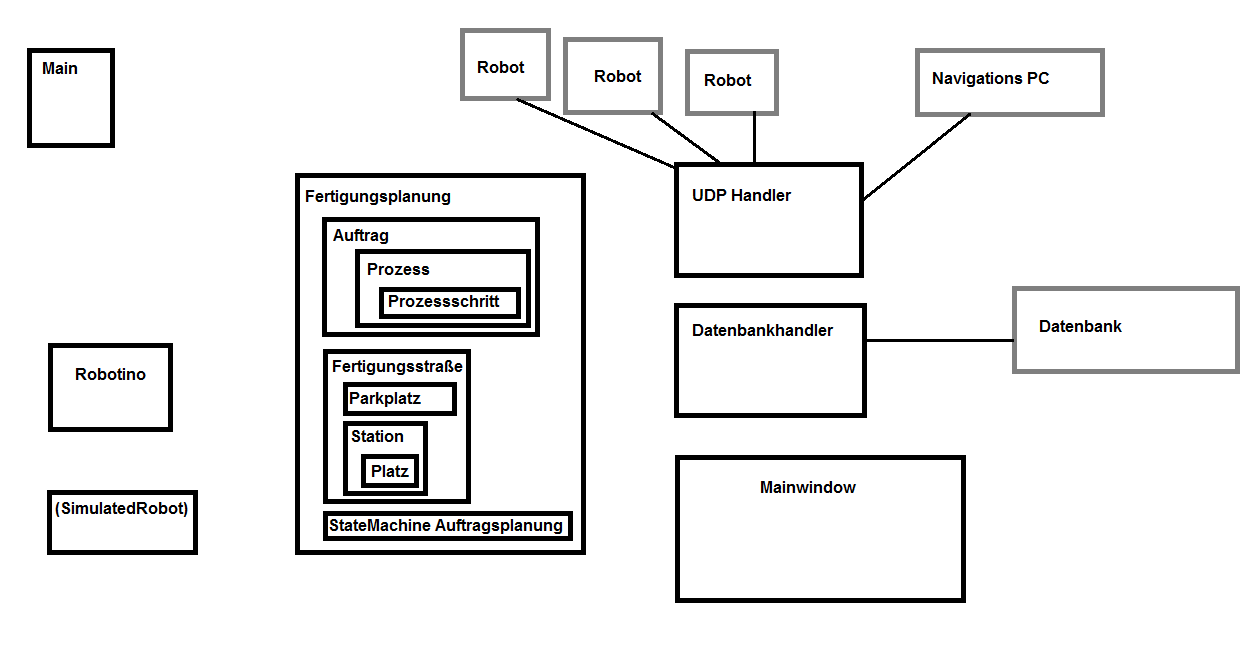
\includegraphics[width=0.9\textwidth]{Abbildungen/Klassendiagramm.PNG}
    \caption{Klassendiagramm}		
    \label{fig:Klassendiagramm}
\end{figure}



\section{Databasehandler}
\section{UDP-Handler} 
\section{Fertigungsplanung}

\begin{figure}[htb]
    \centering
    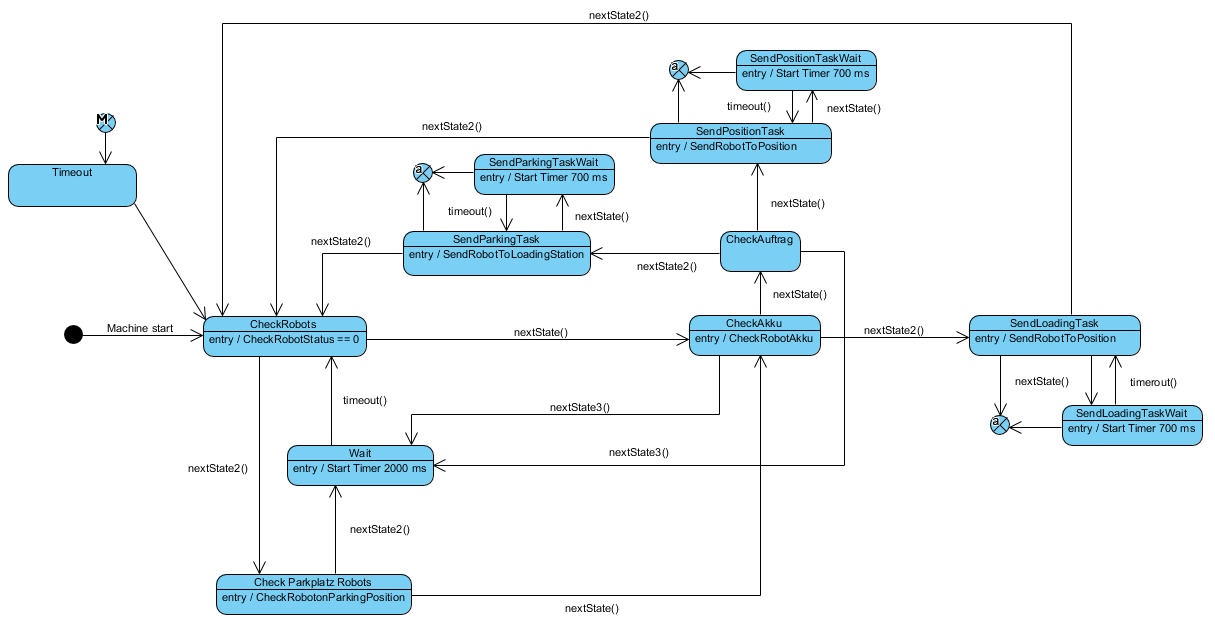
\includegraphics[width=0.9\textwidth]{Abbildungen/Auftragsplanung.PNG}
    \caption{Ablaufdiagramm der Auftragsplanung}		
    \label{fig:Auftragsplanung}
\end{figure}

\section{Mainwindow}
\section{Weitere Klassen}


